


Many sampling efforts for linguistic data on the web are heavily focused on producing results comparable to conventional corpora.  These typically take two forms: those based on URL lists (e.g.\ from search results, as in %~\cite{sharoff2006creating}
BE06~\cite{baker2009be06}, BootCaT~\cite{baroni2004bootcat}), and those formed through crawling (e.g.\ enTenTen\footnote{\url{http://trac.sketchengine.co.uk/wiki/Corpora/enTenTen}},
UKWaC~\cite{ferraresi2008introducing}).

Though initial efforts in web-as-corpus (WaC) focused on the former method %, in part due to concerns over the balance of samples returned, 
many projects are now constructing supercorpora, which may themselves be searched with greater precision than the `raw' web, in line with Kilgarriff's vision of linguistic search engines~\cite{kilgarriff2003linguistic}.  This has led to the proliferation of crawlers such as those used in~\cite{schafer8building} and WebCorp\footnote{\url{http://www.webcorp.org.uk/live/
}}~\cite{renouf2003webcorp}.

% diachronic work with webcorp.
% \cite{kehoe2006diachronic}
% \cite{kehoe2009weaving}

This approach, with its base in a continually-growing supercorpus, parallels the strategy of a monitor corpus~\cite{sinclair1982monitor}, and is applicable to linguistic inquiry concerned with diachronic properties~\cite{kehoe2006diachronic}.
%Even for informal searches, tools for date-based lookup are increasingly (e.g. Google).


Repeated sampling by crawling, whilst balanced linguistically, omits subtler technical aspects that govern consumption of data online, most notably the user's impression of its location, as defined by the URL\@.  Low publishing costs online, paired with increasing corporate oversight and reputation management (both personal\cite{ICT4DBibliography1650} 
and professional\cite{Malaga2000repman}), have lead to a situation where this content is being revised frequently, often without users even noticing.

The nature of within-URL change have been studied from a technical perspective by those interested in managing network infrastructure, compiling digital libraries~\cite{tyler2003librarians}, and optimising the maintenance of search engine databases~\cite{koehler2004longitudinal}.  The needs of these parties are quite aside from those of corpus researchers, however, since they focus around a best-effort database of information, rather than a dependable longitudinal sample with known margins for error.

% ---
Current methods for sampling language change online include:

\begin{itemizeTitle}

    \item[Crawlers/Revisiting] Continuously crawl pages, adding new ones as links are updated and revisiting old ones according to heuristics;
    \item[Diachronic corpora] Build two separate corpora using the same sample design at different points in time;
    \item[Monitor corpora] Continuously add new material to a corpus as it is created, agnostic of change;
    \item[Subsampling supercorpora] Build a large corpus and select documents from it according to a bimodal distribution of document age;
    \item[Feed corpora] Crawl pages on publication date (a form of monitor corpus).

\end{itemizeTitle}


Each of these methods is subject to a number of downsides, making them difficult to use for many scientific purposes, or requiring significant resources and forward-planning (thus putting them out of the hands of most researchers).  Some issues, such as irregular revisiting of pages and the lack of detail stored about network-level metadata, complicate the process of analysis.  Most corpus formats are also not annotated by time, meaning that analysis often requires repeated export and comparison---tools for which must be produced on a case-by-case basis.

% 
% \begin{itemize}
%     \item \textsl{Incremental sampling}---Search engine databases and digital archives are persistent, and may be incrementally updated in a continuous manner whilst still being useful;
%     \item \textsl{Lack of comparability}---A cross-sectional sample of search databses yields documents sampled at various times, with a possible age variation as modelled by the specific type of web page.  This is evidenced well by the relative likelihood of receiving a broken link when searching for current events \textsl{vs.} older scientific articles.
%     \item \textsl{Information-seeking behaviour}---Search engine literature indicates [CITE] that information, when lost from one location, is often available at many others.  This same process is unlikely to be followed, however, if a resource has simply changed, or if a user relies on a small set of web pages as an information resource (such as news sources).
%     \item \textsl{Deliberate `usefulness bias'}---Sources deemed to be pertinent to a search engine's clientelle are sampled more frequently, and thoroughly.  This results in persistence-of-value surrounding high-profile domain names and companies, which dominate the zipfian distribution of web results.
% \end{itemize}
% 


I present here a tool, LWAC, for this form of longitudinal sampling, designed to maximise the comparability of documents downloaded in each sample in terms of their URL rather than content.  To accomplish this, we use a cohort sampling strategy, as illustrated in Figure~\ref{fig:longitudinal:lwac:samples}, to get full coverage over a list of URLs, at the expense of sampling new content.

\begin{figure}[Ht]
    \centering
    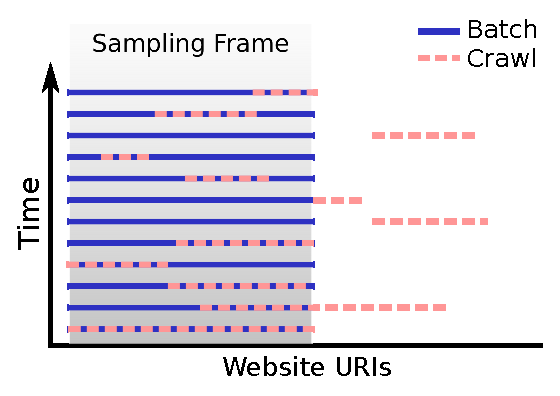
\includegraphics[width=0.6\textwidth]{longitudinal/lwac-samples}
    \caption{URL coverage for batch and crawl}
    \label{fig:longitudinal:lwac:samples}
\end{figure}

This approach allows for reliable re-visits to each member of the sample, and thus the construction of vertically comparable data points, whilst making short-term effects visible by revisiting each link.  Such a sample design should repeat each individual sample as quickly as possible, so as to minimise the time differences between documents within.


This allow a user to investigate how language may change in relation to technical and social events in a way that mimics the experience of many end users, and offers a useful perspective on many epistemic problems of WaC methods, to determine:

\til{Integrate these as an extension of the previous section}

\begin{itemize}
    \item The portions of web pages that typically change as main content regions;
        \vspace{-6pt}
    \item The impact of social feedback and user generated content on page content;
        \vspace{-6pt}
    \item How censorship, redaction and revision affect website contents;
        \vspace{-6pt}
    \item Website resource persistence and its relation to linguistic content;
        \vspace{-6pt}
    \item How institutions' publishing policies affect reporting of current events.
\end{itemize}

LWAC is designed to construct longitudinal samples from URL lists, using only commodity hardware.  It is designed with `full storage' in mind, that is, recording everything about each HTTP session in such a way that it may later be exported and accessed in a parsimonious manner.


LWAC is based around a central corpus store that is indexed both by time and URL\@.  Each sample consists of all datapoints in the corpus, and begins at a specified time: this time is aligned to a sampling interval.

Figure~\ref{fig:longitudinal:lwac:samples} shows the logical structure of the corpus: the blue bars represent each sample.  The primary technical challenge lies in maximising the parallelism of each sample, thus improving the comparability of datapoints therein and allowing for a smaller sampling interval.  Samples that overlap their sampling interval will not be stopped: instead the next sample will be delayed until the next `round' interval.  This eases analysis by ensuring the integrity and temporal alignment of each sample.

Documents are downloaded in a random order, so as to avoid systematic variation in sample times across links.



\subsection{Design \& Implementation}


\begin{figure}[Ht]
    \centering
    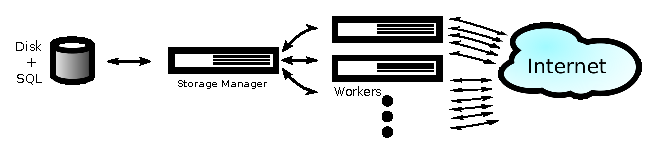
\includegraphics[width=\textwidth]{longitudinal/lwac-arch}
    \caption{System Architecture}
    \label{fig:longitudinal:lwac:arch}
\end{figure}


In order to perform the parallel retrieval stage quickly, LWAC is constructed as a distributed system, with a series of workers performing the page retrieval and passing batches of data to an offline system for further processing.  This architecture, shown in Figure~\ref{fig:longitudinal:lwac:arch} is extensible until the limit of contention for the storage manager's network connection is reached, which in practice is encountered at many tens of worker nodes.  In addition to the use of multiple workers, each worker performs many parallel requests\footnote{The portion of LWAC used for parallel request management is available separately at \url{https://rubygems.org/gems/blat}}.

The storage manager is responsible for all scheduling and data integrity: workers are treated as (relatively) untrusted actors, and allocated batches of links on request.  The scheduling system monitors performance of each worker, and dynamically computes a timeout for work units: exceeding this timeout will see the batch of links re-assigned to another worker.  This system allows for great flexibility in workers, which may vary in batch size and connection throughput.

The storage manager is also responsible for enforcing atomicity of jobs and of the underlying corpus.  This is enforced using a check-out system: workers check out batches of links that remain allocated until they are returned, completed, by the same worker.  When a sample is complete, it is `sealed' on disk to prevent further edits, and the scheduler instructs workers to sleep until the next sample time.


\begin{lstlisting}[language=,caption={Corpus directory structure on-disk},label=lst:longitudinal:lwac:corpusformat]
root/
root/database.db
root/state
root/files/sample_id/sample
root/files/sample_id/1/2/3/456
\end{lstlisting}

% The metadata database (if using SQLite3)
% The state of the current sample. This is stored as a serialised ruby object so that a sample may be resumed later if the server is stopped.
% A list of sample ID folders containing:
% A file describing the properties of this sample as a serialised ruby Sample object
% A structure of directories describing link IDs, each of which has up to N files within it (as defined in the server config). This structure uses the first characters of the ID to nest directories in order to avoid filesystem limits on inode size and speed up random access, i.e.: 0/1/1 0/1/2 0/1/3 0/2/1 0/2/2 0/2/3 etc.


Data storage in the system is split between metadata, stored in an SQL database, and website sample data itself, which is stored as raw HTTP response data in a versioned structure on disk.  The storage format is optimised for large samples, and is nested in order to avoid common filesystem limits (as shown in Listing~\ref{lst:longitudinal:lwac:corpusformat}
).  LWAC does not enumerate URLs in memory, meaning there is no hard limit on corpus size---instead it incrementally loads links as requested by the workers.  This means that memory usage is limited to the maximum batch size within the system.

Workers are able to imitate the behaviour of end users' browsers as much as possible, so as to avoid search engine optimisation and user-agent detection tactics.  They are able to provide cookies and request headers commensurate with a web browser, and follow redirects to similar depths.  This behaviour is passed as part of the work unit itself, and so is configured centrally.

Workers are able to enforce limits on MIME type and file size, ensuring that documents are not downloaded if they are incompatible with further evaluation stages.

After downloads have occurred, data may be retrieved for analysis in a variety of formats using the included export tool.  Export is possible at one of three levels: all data, individual samples (all datapoints at a given time), or individual datapoints (across all times).


Metadata is stored about network-level properties such as timeouts and latencies, as well as URL properties (link length, etc.) and HTTP headers.  The original request parameters and sample design are also presented in the same structure, allowing corpora to be somewhat self-documenting.  Appendix~\ref{sec:appx:fields} shows the object hierarchy of page data.


Exports are performed by filtering data using a series of expressions.  These data are then passed to formatting expressions, which are able to normalise display formats for analysis, before calling a number of pluggable formatting modules.  Current formats supported are:

\begin{itemize}
    \item CSV format with one-row-per-datapoint or per-sample;
    \item A collection of CSV files, split per-sample;
    \item JSON collections, for import into tools such as MongoDB;
    \item Arbitrary text output using the ERB template format.  Supports server, sample and datapoint level exporting;
    \item XML, transformed from the original input parameters using XSLT.
\end{itemize}



\subsubsection{Resource Usage}

LWAC is designed to handle corpora of theoretically infinite size, and uses a pipelined design to avoid enumerating its corpus members.  In practice the limit on corpus size is imposed by the SQL server used.

Memory usage is $O(1)$ for both the storage server (which backs all of its corpus data with the disk) and the client (which only ever loads as many datapoints as number of parallel connections).  Ultimate limits are defined by the batch size chosen for workers:

\begin{itemize}
    \item Server: $(\textit{clients} \times \textit{batch\_size} \times \textit{link\_size}) + (\textit{batch\_size} \times \textit{max\_resource\_size})$
    \item Client: $\textit{in\_progress} \times \textit{max\_resource\_size}$ (using disk cache)
\end{itemize}

Workers use static quantities of disk, equal to the maximum download size of each page multiplied by the batch size.  Disk usage for the storage controller is $O(N)$,  though the storage format is well suited to deduplication using symlinks to point to previous data.


\subsection{Performance}
Ultimate performance is dependent on a number of factors:

\begin{itemize}
    \item The number of worker machines used;
    \item The number of connections per worker;
    \item Worker network speeds;
    \item Latency of DNS and web servers.
\end{itemize}

The last of these implies gradual degradation of performance as links rot.  Performance figures stated here are therefore for the `best case' scenario where links are all available from fast servers.


\subsubsection{Artificial}


\begin{figure}[Ht]
    \centering
    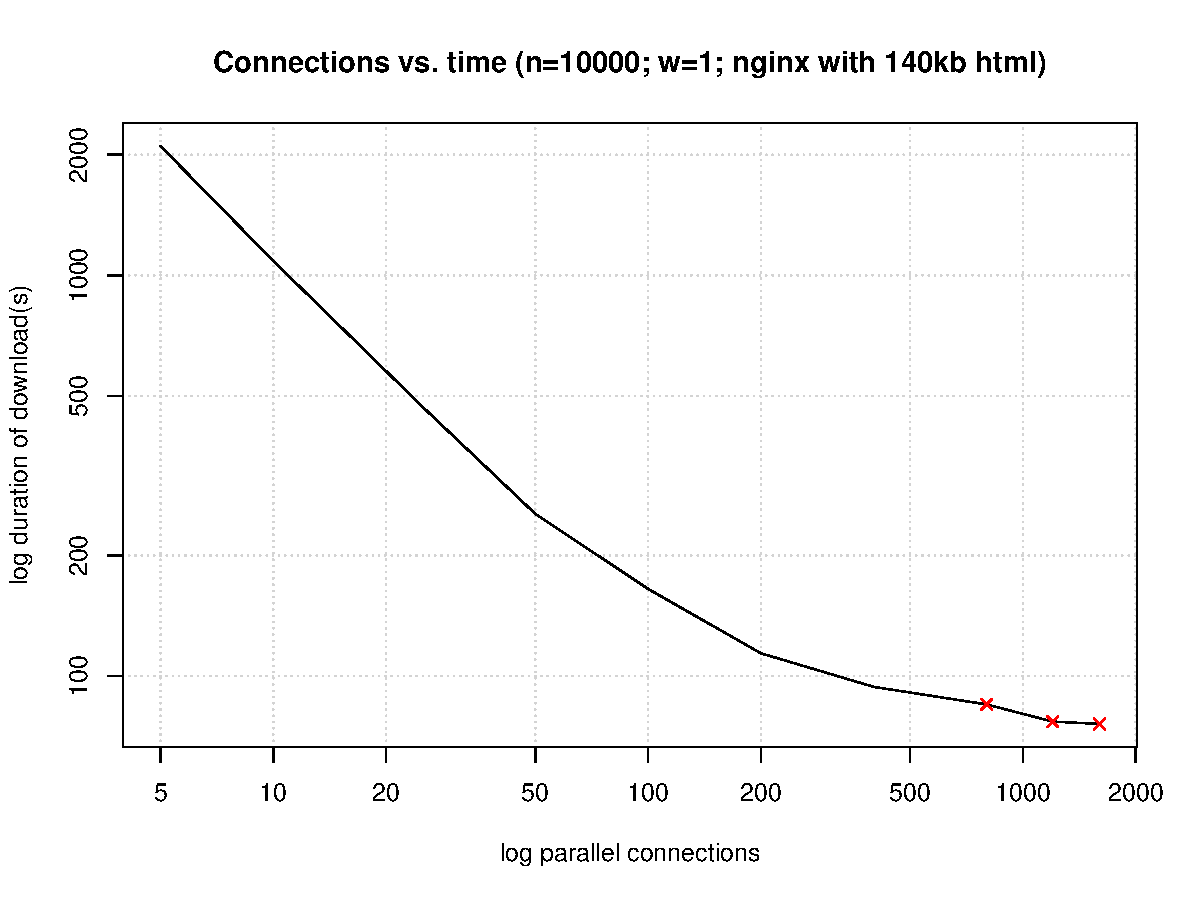
\includegraphics[width=\textwidth]{longitudinal/lwac-parallelrate}
    \caption{Download speeds for one worker for various levels of parallelism}
    \label{fig:longitudinal:lwac:parallelrate}
\end{figure}

Figure~\ref{fig:longitudinal:lwac:parallelrate} shows the download rate for 140KiB HTML files served over 100Mbit ethernet using the Nginx web server.  This server configuration was designed to offer high-performance yet still be representative of common web deployments\footnote{Nginx is known for its ability to serve many users at once, and ``[a]ccording to Netcraft, nginx served or proxied 21.64\% busiest sites in May 2015.''---\url{http://nginx.org/en/}}.

The performance of parallel downloads is largely constrained by the platform, in this case the Linux 2.6 kernel.  Downloads are reliable until roughly 700 parallel connections are used, beyond which requests are dropped locally as half-open sockets are closed.  Until this point performance is roughly log-linear, with 100,000 requests taking just 100 seconds with 500 parallel connections.  For subsequent tests, 400 connections per worker machine were used.


\begin{figure}[Ht]
    \centering
    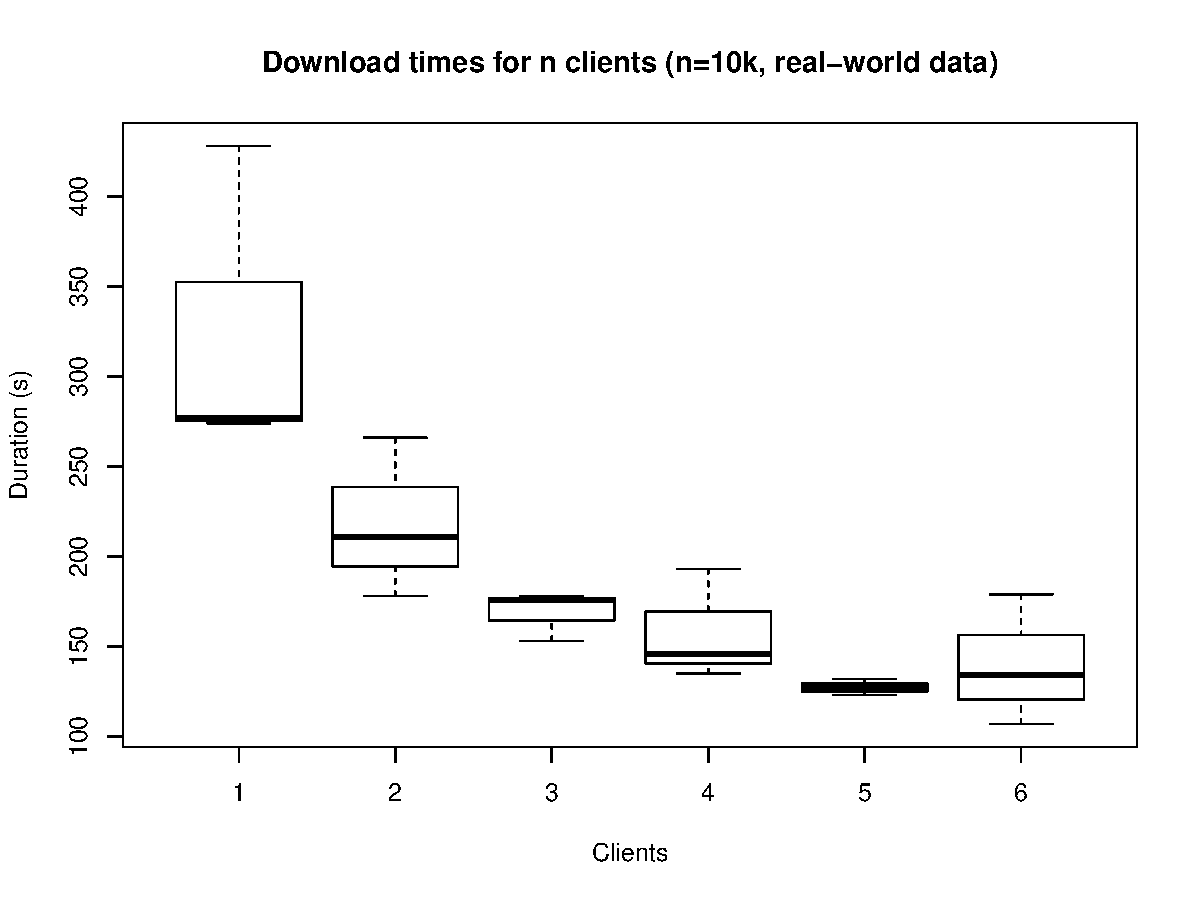
\includegraphics[width=\textwidth]{longitudinal/lwac-clientrate}
    \caption{Download speeds for 10,000 real-world HTML documents.}
    \label{fig:longitudinal:lwac:numclients}
\end{figure}


Selecting the number of worker machines required for a deployment is a tradeoff between many factors, particularly cost and download rate\footnote{Reliability and physical location are also likely to influence results, especially where geography affects the contents of pages}.  As the server is responsible for all co-ordination, the speed improvements seen when adding worker machines is nonlinear, eventually plateauing where the overhead of the batch request equals the difference in time between requests made by $n$ and $n + 1$ workers.

Figure~\ref{fig:longitudinal:lwac:numclients} shows the overall download times for the same dataset when using differing numbers of workers.  Workers were all connected to the storage manager via 100Mbit ethernet (minimising contention), and were making requests via the same link to a local test machine.  As expected, the improvements soon plateau, though there is a large amount of variance---larger batch sizes and a larger test corpus are expected to show further improvement with $n > 6$.  This plateau may be expected to occur earlier if workers are connected via relatively low-bandwidth links (for example, if they are connected over long distances via the internet or a VPN).





\subsubsection{Real-world}

In order to test retrieval performance in a real-world scenario, a test deployment was constructed consisting of three clients, each making 400 parallel connections.  Each was running Linux 2.6 connected to the storage manager using a 100Mbit ethernet link, and to the internet using Lancaster University's tier-1 fibre connection.  This setup was designed to be within reach of many academic users, who are likely to have bandwidth allocations exceeding the sites that they visit, yet have limited access to hardware.


The 228,000 URLs used were sourced using BootCaT, making 4600 requests to the Bing search engine and retrieving 50 links per request.  This resulted in a corpus size of 14.9GiB, which, after boilerplate removal, yielded 588 million words.


\begin{figure}[Ht]
    \centering
    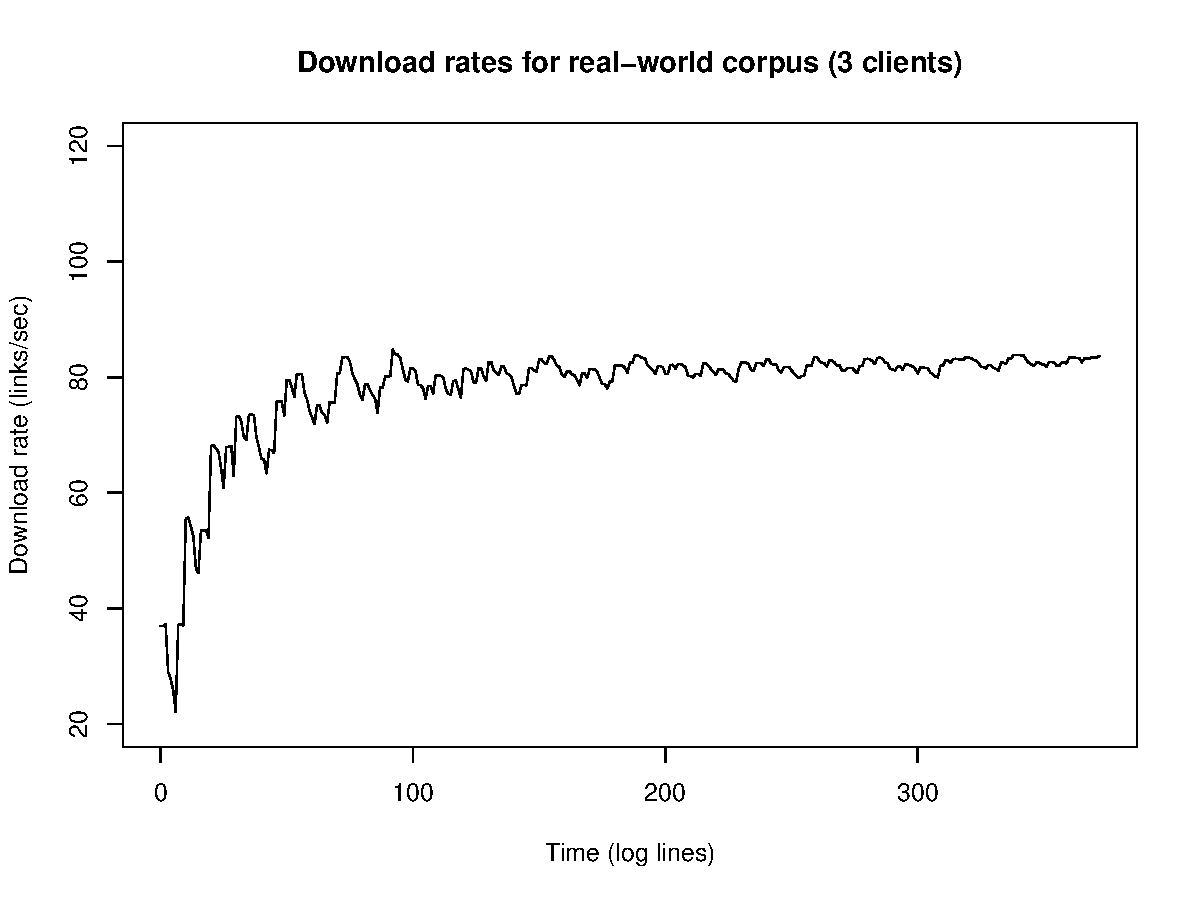
\includegraphics[width=\textwidth]{longitudinal/lwac-realrate400}
    \caption{Download rate over time for real-world BootCaT derived dataset.}
    \label{fig:longitudinal:lwac:realrate400}
\end{figure}

The throughput over time is shown in Figure~\ref{fig:longitudinal:lwac:realrate400}.  This data was summarised by examining the logs of the storage manager, and thus represents rate calculated after each worker has checked in its batch---hence the pattern of jagged increases followed by gradual decay.  Larger spikes are seen towards the left hand side due to synchronisation of the check-ins by clients: eventually variations in batch retrieval times cause these to disperse and smooth out.  This deployment can be seen to plateau at roughly 80 links per second (roughly 288,000 per hour), meaning the full 228,000 page corpus was retrieved in roughly 45 minutes.

Using this deployment would mean that retrieval of a corpus the size of the BNC is possible in around eight minutes; a ukWaC\cite{ferraresi2008introducing} copy would take 2.5 hours (or 17 if using the pre-filtered url list), and DECOW2012\cite{schafer2012building} would take 24 hours.





\subsubsection{Etiquette}
Ordinarily, crawlers are expected to adhere to well-acknowledged guidelines regarding page retrieval, revisit times, and link traversal.  LWAC ignores these by design, due to a number of factors that differentiate it from standard crawlers.

Firstly, the integrity of the returned samples is impossible to validate if they are not reliably retrieved.  Any missing data would have to be imputed, reducing its scientific value and complicating the process of analysing results.

Secondly, though this is largely under the control of the user, it is expected that links will not be visited so regularly as to significantly increase load on a given server.  Most effects requiring longitudinal analysis take place over a relatively long period of time that does not warrant short sample periods.

Finally, LWAC's link selection is unlikely to include many pages hosted on the same server.  This is not guaranteed, however, for web-wide longitudinal analyses each `hit' by LWAC is not going to result in immediate successive hits to the same server, as it would with a crawler that navigates pages.  Where this is violated, it is of course up to the user to mitigate any load to the web server.  LWAC's randomisation of the order of link traversal also helps mitigate this, as it reduces the chances of a set of links co-occuring systematically in each sample.

Though it is possible to perform DDOS-style attacks using LWAC, the use-case for which it was designed is unlikely to violate the principles adhered to by existing crawlers.






% Currently, workers do not interpret JavasScript or construct a DOM

